\nopagebreak
\begin{figure*}[]
	\sidesubfloat[First subfigure]{%
	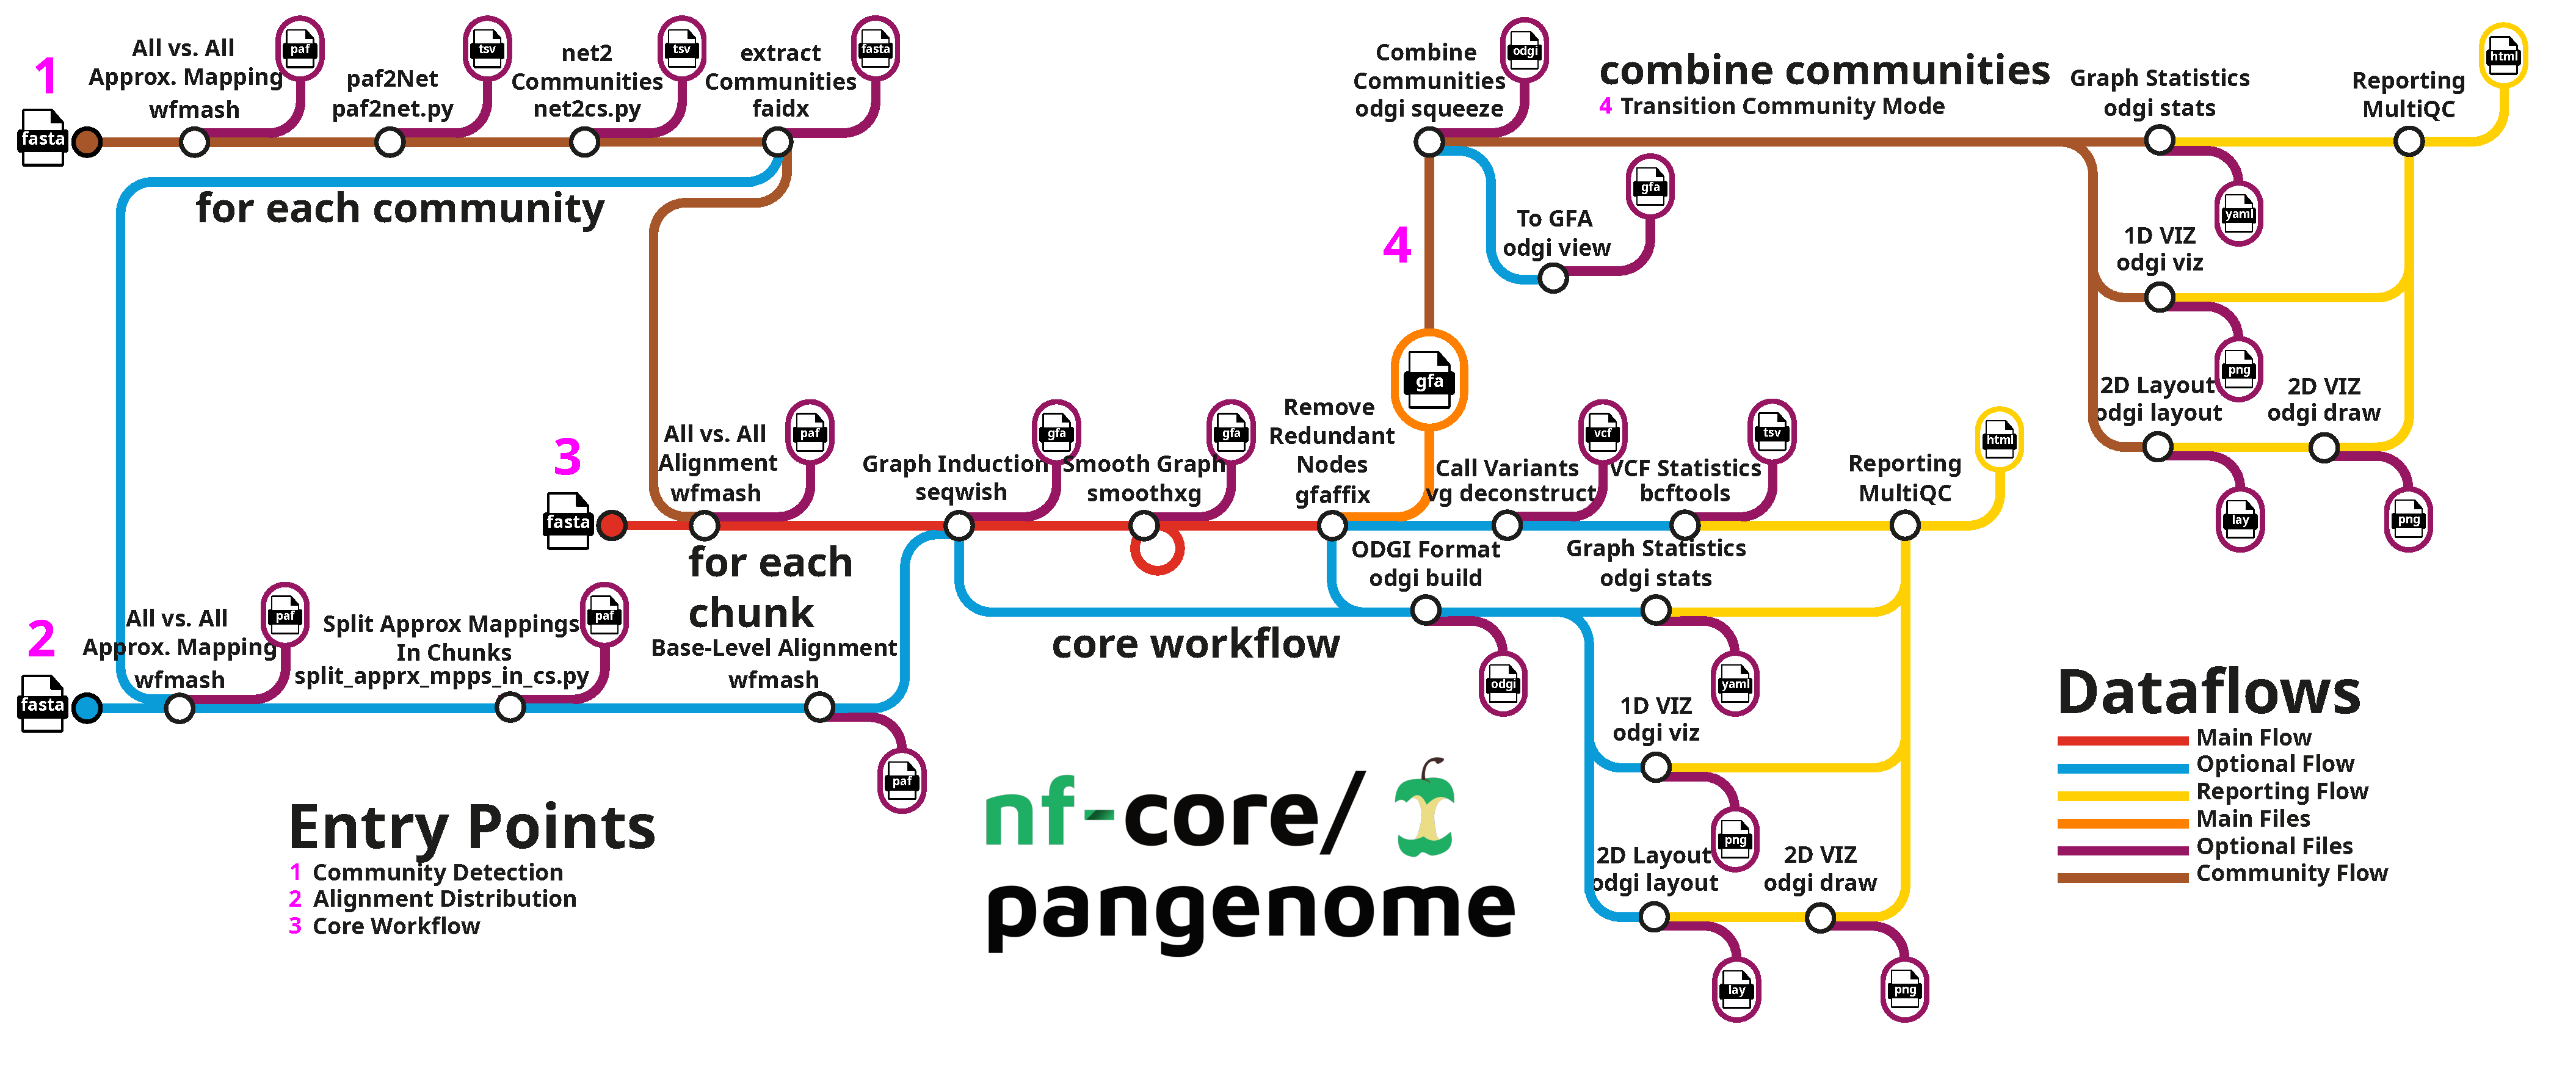
\includegraphics[width=\textwidth]{fig/pangenome_workflow.pdf}
	\label{fig1:workflow}
	}
	\hfill
	\sidesubfloat[Second subfigure]{%
		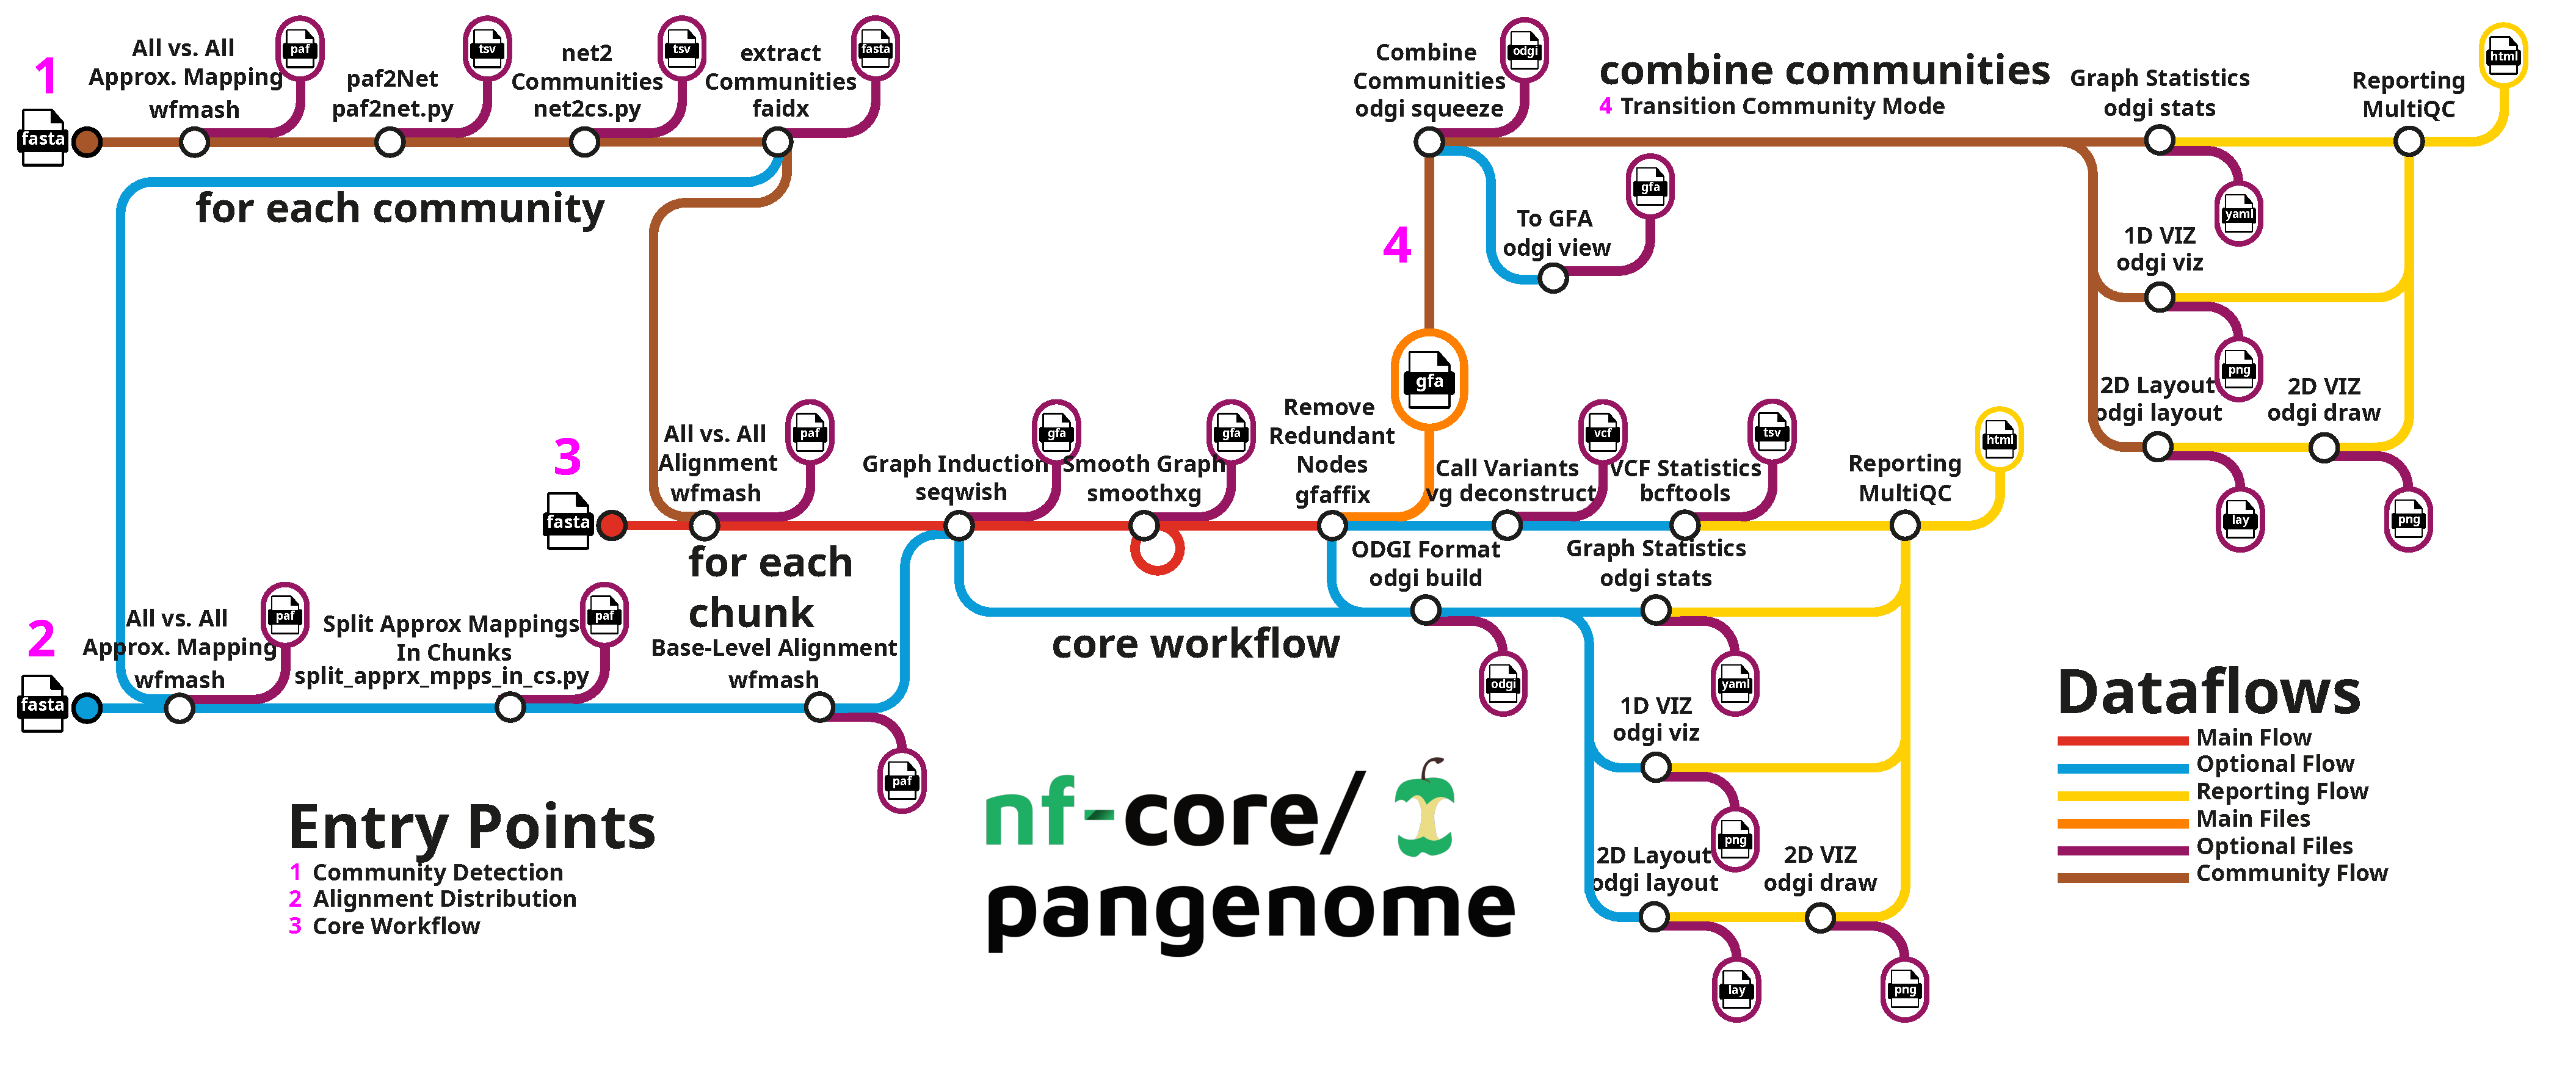
\includegraphics[width=\textwidth]{fig/pangenome_workflow.pdf}
		\label{fig1:worky}
	}
	\caption{\textbf{(a)} Schematic representation of the nf-core/pangenome workflow processes and detailed analysis steps. The input consists of one FASTA file containing all sequences. The pipeline comes with 3 major entry points: Community detection (1), alignment distribution (2), and core workflow (3). Optional community detection (1) is performed on the input sequences. If selected, the heavy all-to-all baise-pair level alignments (2) can be split into problems of equal size. nf-core/pangenome’s core workflow (3) is a direct mirror of PGGB. If running in community mode, all communal graphs are combined into one (4) and the subsequent quality control subworkflow is executed. The output is a pangenome graph in GFA format.
	}
	\label{fig1:panel}
\end{figure*}